\section{Lista de Figuras}
\begin{figure}[h]
\vspace{0.1in}
\begin{center}
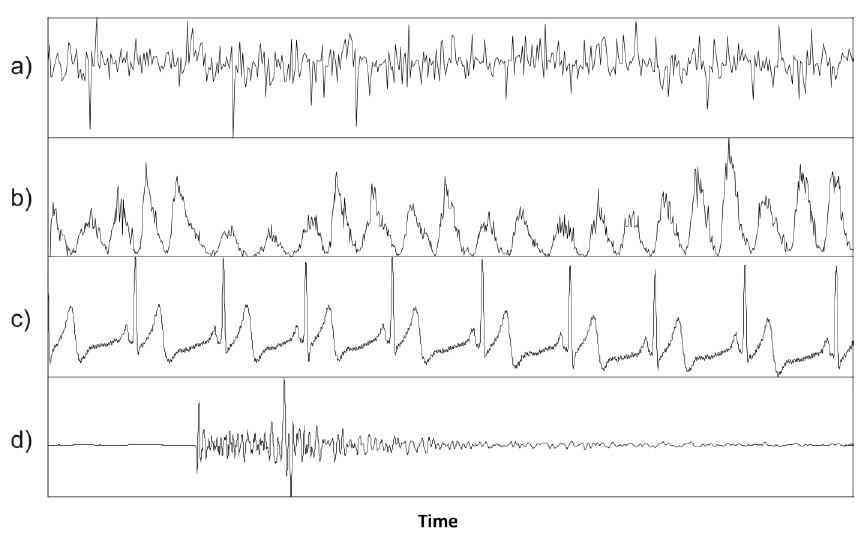
\includegraphics[scale=0.6]{timeSeries.png}\\%
\end{center}
\caption{Ejemplos de Series Temporales}
\label{arm:fig1}
\end{figure}
\begin{figure}[h]
\vspace{0.1in}
\begin{center}
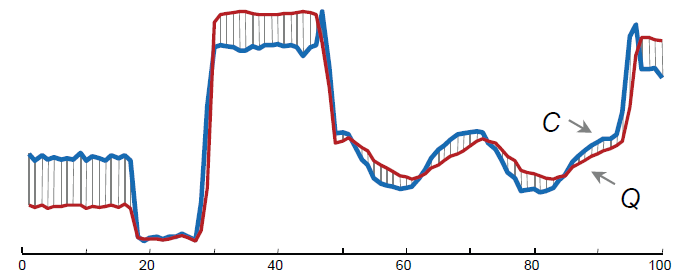
\includegraphics[scale=0.6]{euclidean.png}\\
\end{center}
\caption{Visualizaci\'on de la distancia Euclidiana de dos series temporales.}
\label{arm:fig2}
\end{figure}
\begin{figure}[h]
\vspace{0.1in}
\begin{center}
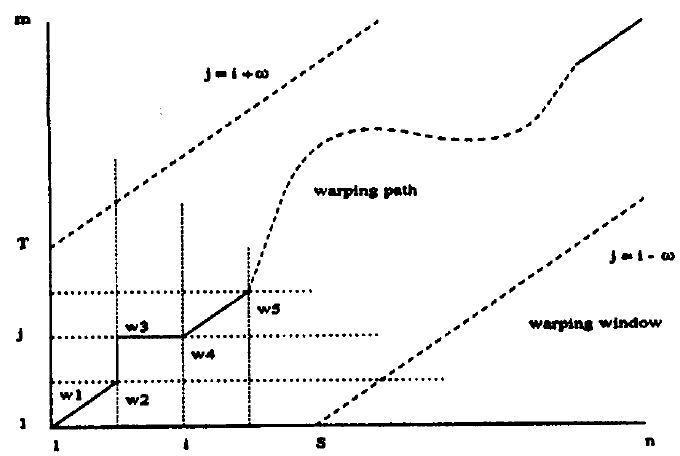
\includegraphics[scale=0.6]{dtw.png}\\
\end{center}
\caption{Visualizaci\'on de la minimizaci\'on de una ruta en DTW.}
\label{arm:fig3}
\end{figure}
\begin{figure}[h]
\vspace{0.1in}
\begin{center}
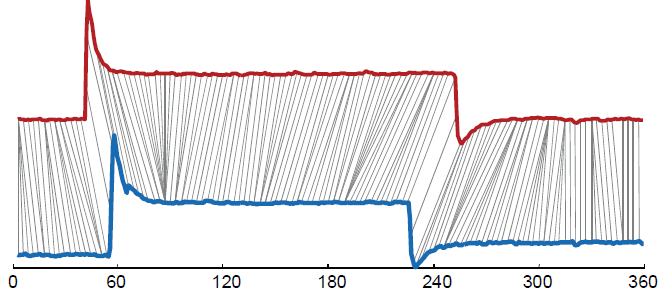
\includegraphics[scale=0.6]{dtw2.png}\\
\end{center}
\caption{Visualizaci\'on del calculo de DTW.}
\label{arm:fig4}
\end{figure}
\begin{figure}[h]
\vspace{0.1in}
\begin{center}
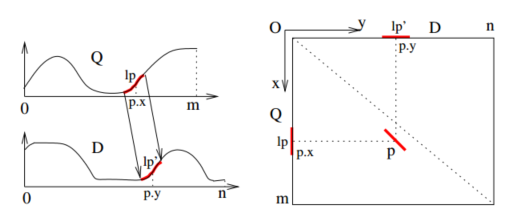
\includegraphics[scale=0.6]{spade.png}\\
\end{center}
\caption{Ejemplo del c\'alculo de LPM.}
\label{arm:fig5}
\end{figure}
\begin{figure}[h]
\vspace{0.1in}
\begin{center}
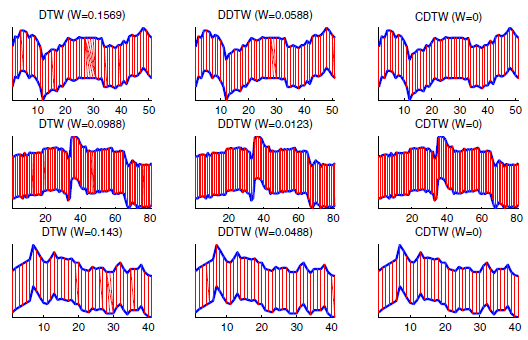
\includegraphics[scale=1]{cdtw.png}\\
\end{center}
\caption{Visualizaci\'on de deformaciones innecesarias en DTW.}
\label{arm:fig6}
\end{figure}
\begin{figure}[h]
\vspace{0.1in}
\begin{center}
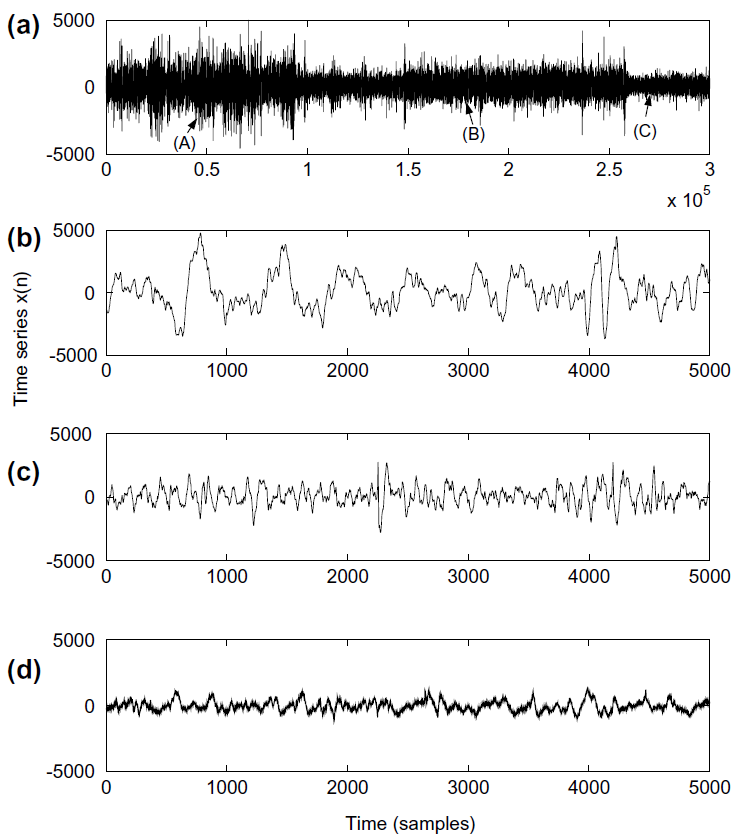
\includegraphics[scale=0.6]{brainsignal.png}\\
\end{center}
\caption{Ejemplo de ruido en las se\~nales de un electoencefalograma.}
\label{arm:fig7}
\end{figure}